\chapter{Machine learning and Artificial Neural Network}
\label{sec:ml}

\epigraph{``I have the shape of a human being and organs equivalent to those of a human being. My organs, in fact, are identical to some of those in a prosthetized human being. I have contributed artistically, literally, and scientifically to human culture as much as any human being now alive. What more can one ask?''}{Isaac Asimov, The Complete Robot }

Machine Learning (ML) and more specifically Neural Network (NN) are a family of data-driven algorithm. They are used to model complex distribution from a finite dataset to extract a generalist behavior where they learn, adapt their intrinsic parameters, interactively by computing the performance or \textit{loss} on those dataset. They take advantage of simple microscopic operation such as \textit{if condition}, non-continuous but differentiable function like \textit{ReLU}. Through optimizer and the combination of those microscopic operation, they can yield complex and precise behavior.

They are now widely used in a wide variety of domain including natural language processing, computer vision, speech recognition and, the subject of this thesis, scientific studies.


They are now widely used in particle physics, either as the main algorithm or as secondary algorithm, for event reconstruction, event classification, waveform reconstruction, etc... Domains where the underlying physic and detector process is complex and highly dimensional. Physicists have traditionally used algorithms where simplification or assumption were made (a good example is the algorithm presented in section \ref{sec:juno:reco}) machine learning could refine and take into account those effects, providing that they have enough data and computing power, thus the appeal for physicist.


\section{Boosted Decision Tree (BDT)}
\label{sec:ml:bdt}

One of the most classic machine learning algorithm used in particle physics is Boosted Decision Tree \cite{breiman_classification_2017} (or more recently Gradient Boosting Machine \cite{friedman_greedy_2001}). The principle of BDT is fairly simple : Based on a set of observables, a serie of decisions, represented as node in a tree, are taken by the algorithm. Each decision point, or node, takes its decision based on a set of trainable parameters leading to a subtree of decision. The process is repeated until it reach the final node, yielding the prediction. A simplistic example is given in figure \ref{fig:ml:bdt}.

\begin{figure}
  \centering
  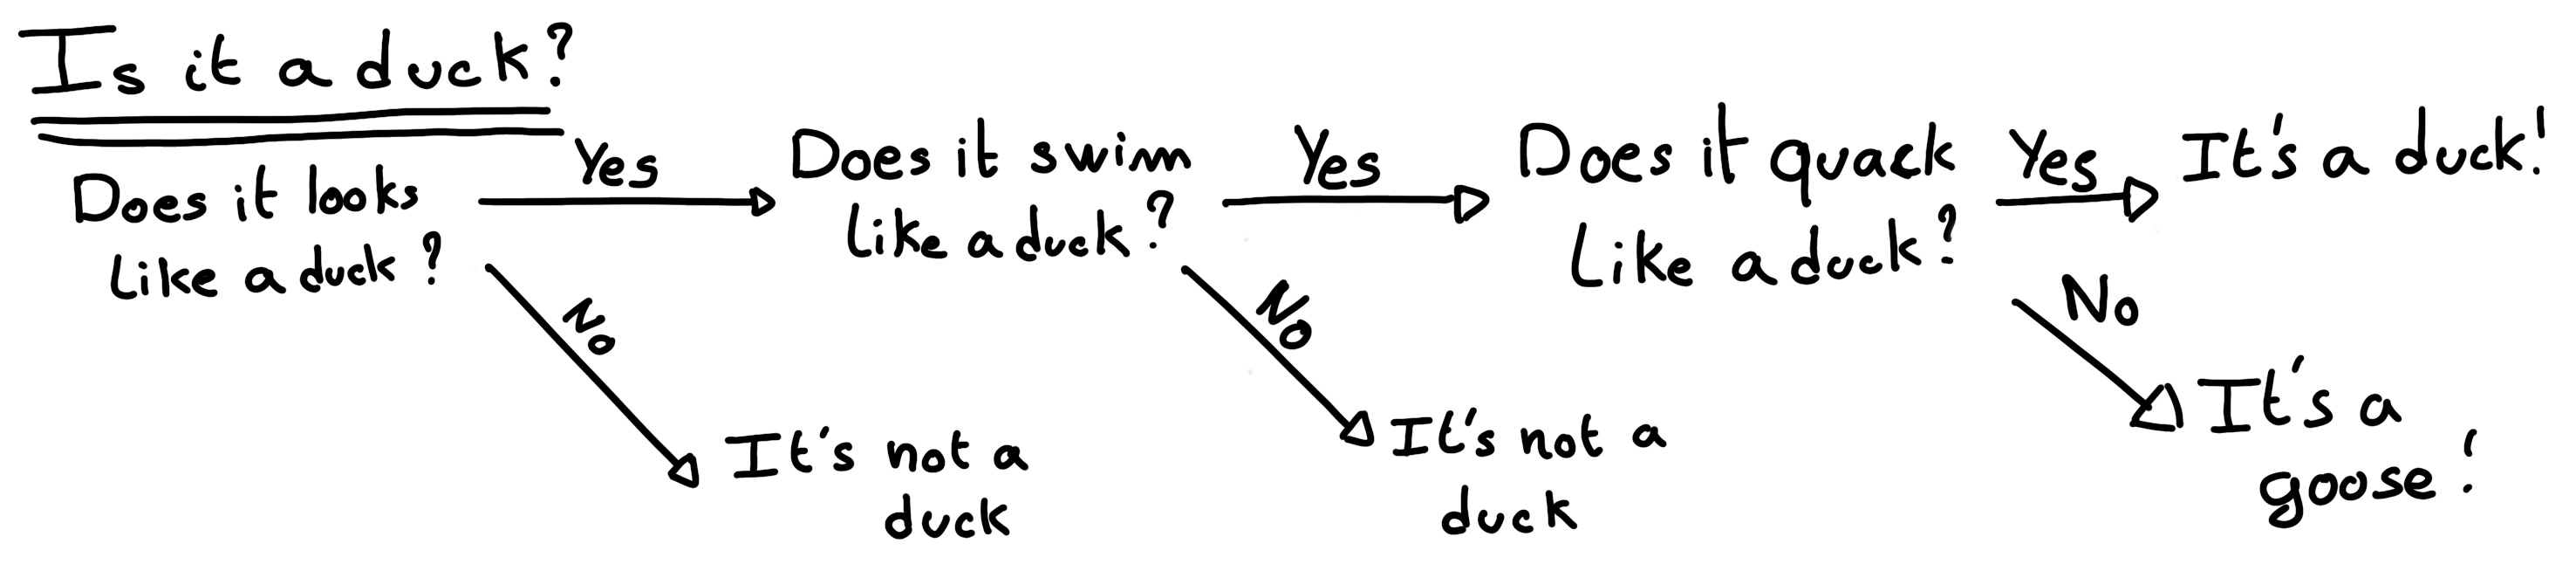
\includegraphics[width=\linewidth]{images/ml/Bdt.jpg}
  \caption{Example of a BDT that determine if the given object is a duck}
  \label{fig:ml:bdt}
\end{figure}

The training procedure follow a simple score reward procedure. During the training phase the prediction of the BDT is compared to a known truth about the data. The score is then used to backpropagate corrections to the parameters of the tree. Modern BDT use gradient boosting where the gradient of the loss is calculated for each of the BDT parameters. Following the gradient descent, we can reach the, hopefully, global minima of the loss for our set of parameters.

\section{Artificial Neural Network (NN)}

One other big family of machine learning algorithm is the Artificial Neural Networks (ANN) more commonly designated as Neural Networks (NN). The idea of developing automates which component mimic, in a simplistic way, the behavior of biological neurons emerge in 1959 with the paper ``\textit{What the Frog's Eye Tells the Frog's Brain}'' \cite{lettvin_what_1959}. They develop an automate where each component possess an \textit{activation function}. Each one of those component then transmit it's information to the other following a certain efficiency or \textit{weight}.
Those works influenced scientist and notably Frank Rosenblatt who published in 1958 what is considered the first neural network model the perceptron \cite{rosenblatt_perceptron_1958}.


Modern neural network still nowadays use the neuron metaphor to represent neural network, but approach them as a graph where the nodes are neurons possessing an activation function and edges holding the weights between those nodes. Most of the modern neural network work with the principle of neurons layers. For example the most basic, fully connected set of layer is a set where each layers possessing the same activation function $F$ and the connection between two layers as a tensor $T^{i}_{j}$ where $i$ is the index of the precedent layer and $j$ the index of the next layer. The propagation from the layer $I$ to $J$ is then described as
\begin{equation}
  \label{eq:ml:fully-connected}
  J_{j} = F_J(T_{j}^{i} I_{i} + B_j)
\end{equation}
where the learning parameters are the tensor $T_j^i$ and the bias tensor $B_j$. This is the fundamental component of the Fully Connected Deep NN (FCDNN) family presented in section \ref{sec:ml:fcdnn}. Most of the modern neural network use gradient descent to optimize their parameters, i.e. the gradient of the parameter $\theta$ in respect of the loss function $\mathcal{L}$ is subtracted to it
\begin{equation}
  \theta_{i+1} = \theta_i - \frac{\partial \theta}{\partial \mathcal{L}}
\end{equation}
$i$ being the training iteration index. This needs the expression of $\mathcal{L}$ dependent of $\theta$ to be differentiable, thus the layer and their activation function also need to be differentiable. This simple gradient descent, designated as Stochastic Gradient Descent (SGD), can be completed with first and second order momentum like with the Adam optimizer \cite{kingma_adam_2017}.

This description of neural networks as layer introduced the principle of \textit{depth} and \textit{width}, the number of layers in the NN and the number of neurons in each layer respectively.

\subsection{Fully Connected Deep Neural Network (FCDNN)}
\label{sec:ml:fcdnn}

Fully Connected Deep Neural Network (FCDNN) architecture is the natural evolution of the Perceptron. The input data is represented as a first order tensor $I_j$ and then fed forward to multiple fully connected layers (Eq \ref{eq:ml:fully-connected}) as presented in the figure \ref{fig:ml:fcdnn}. Most of the time, the classic ReLU function
\begin{equation}
  \label{sec:ml:relu}
  \mathrm{ReLU}(x) = \begin{cases}
    x & \mathrm{if} ~ x \geq 0 \\
    0 & \mathrm{otherwise}
  \end{cases}
\end{equation}
as activation function. Prelu and Sigmoid are also popular choices


\begin{minipage}{0.5\linewidth}
  \begin{equation}
    \label{sec:ml:sigmoid}
    \mathrm{Sigmoid}(x) = \frac{1}{1+ e^{-x}}
  \end{equation}
\end{minipage}
\begin{minipage}{0.5\linewidth}
  \begin{equation}
    \label{sec:ml:prelu}
    \mathrm{PReLU}(x) = \begin{cases}
      x & \mathrm{if} ~ x \geq 0 \\
      \alpha x & \mathrm{otherwise}
    \end{cases}
  \end{equation}
\end{minipage}


The reasoning behind ReLU and PReLU is that with enough of them, you can mimic any continuous function as illustrated in figure \ref{fig:ml:relu-mimic}. Sigmoid is more used in case of classification, its behavior going hand in hand with the Cross Entropy loss function used in classification problems.

\begin{figure}[ht]
  \begin{subfigure}[b]{0.48\textwidth}
    \centering
    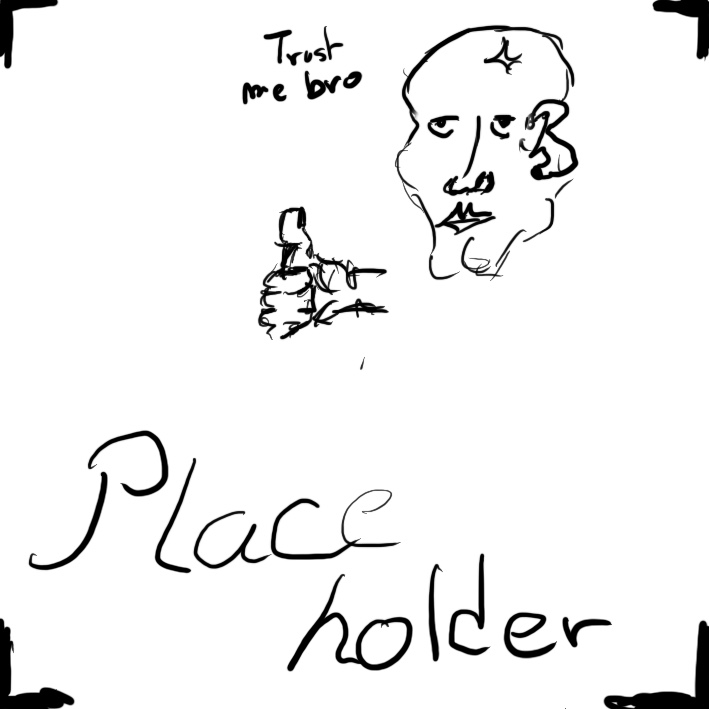
\includegraphics[height=6cm]{images/placeholder.jpg}
    \caption{Schema of a FCDNN}
    \label{fig:ml:fcdnn}
  \end{subfigure}
  \hfill
  \begin{subfigure}[b]{0.48\textwidth}
    \centering
    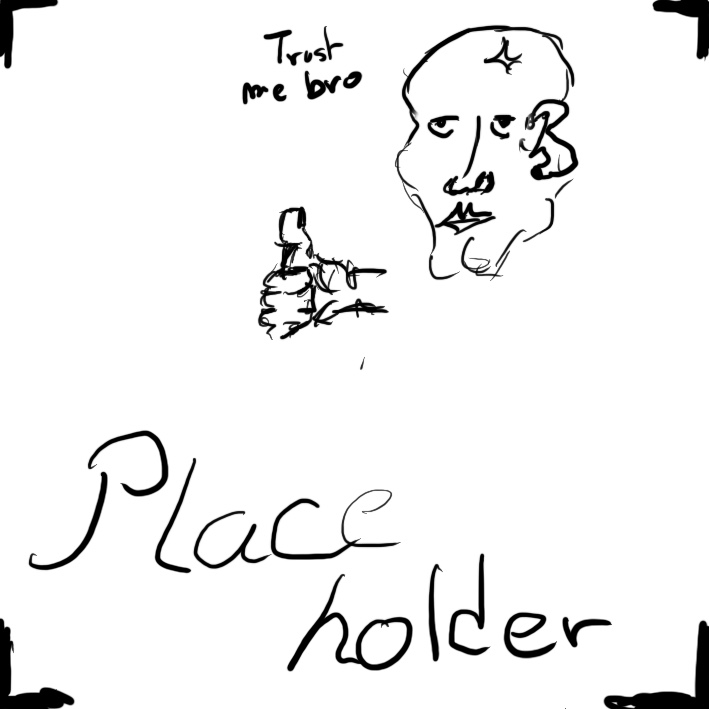
\includegraphics[height=6cm]{images/placeholder.jpg}
    \caption{Illustration of a composition of ReLU matching a function}
    \label{fig:ml:relu-mimic}
  \end{subfigure}
\end{figure}

Due to its simplicity, FCDNN are also used as basic pieces for more complex architecture such as the CNN and GNN that will be presented in the next section.

\subsection{Convolutional Neural Network (CNN)}

\subsection{Graph Neural Network (GNN)}

\subsection{Adversarial Neural Network (ANN)}

\subsubsection{Generative Adversorial Network (GAN)}

\subsubsection{Reinformcement Learning (RL)}

\subsubsection{Random Search (RS)}

\subsubsection{Bayesian Optimization}
